\section{Gestión visual de procesos}

\textit{Kanban} o gestión visual de procesos es un método de gestión de proyectos que se originó en la industria
manufacturera japonesa, específicamente en \textit{Toyota}, como una forma de mejorar la eficiencia de la producción y
que se encuentra fuertemente implantado dentro de la industria del desarrollo de software~\cite{book_anderson_2010}.

El término significa ``tarjeta visual'' en japonés, y el método se basa en el uso de tarjetas visuales para
representar tareas en un tablero, permitiendo a los miembros del equipo ver el estado del progreso del trabajo de un
simple vistazo.

\begin{figure}[ht]
    \begin{center}
        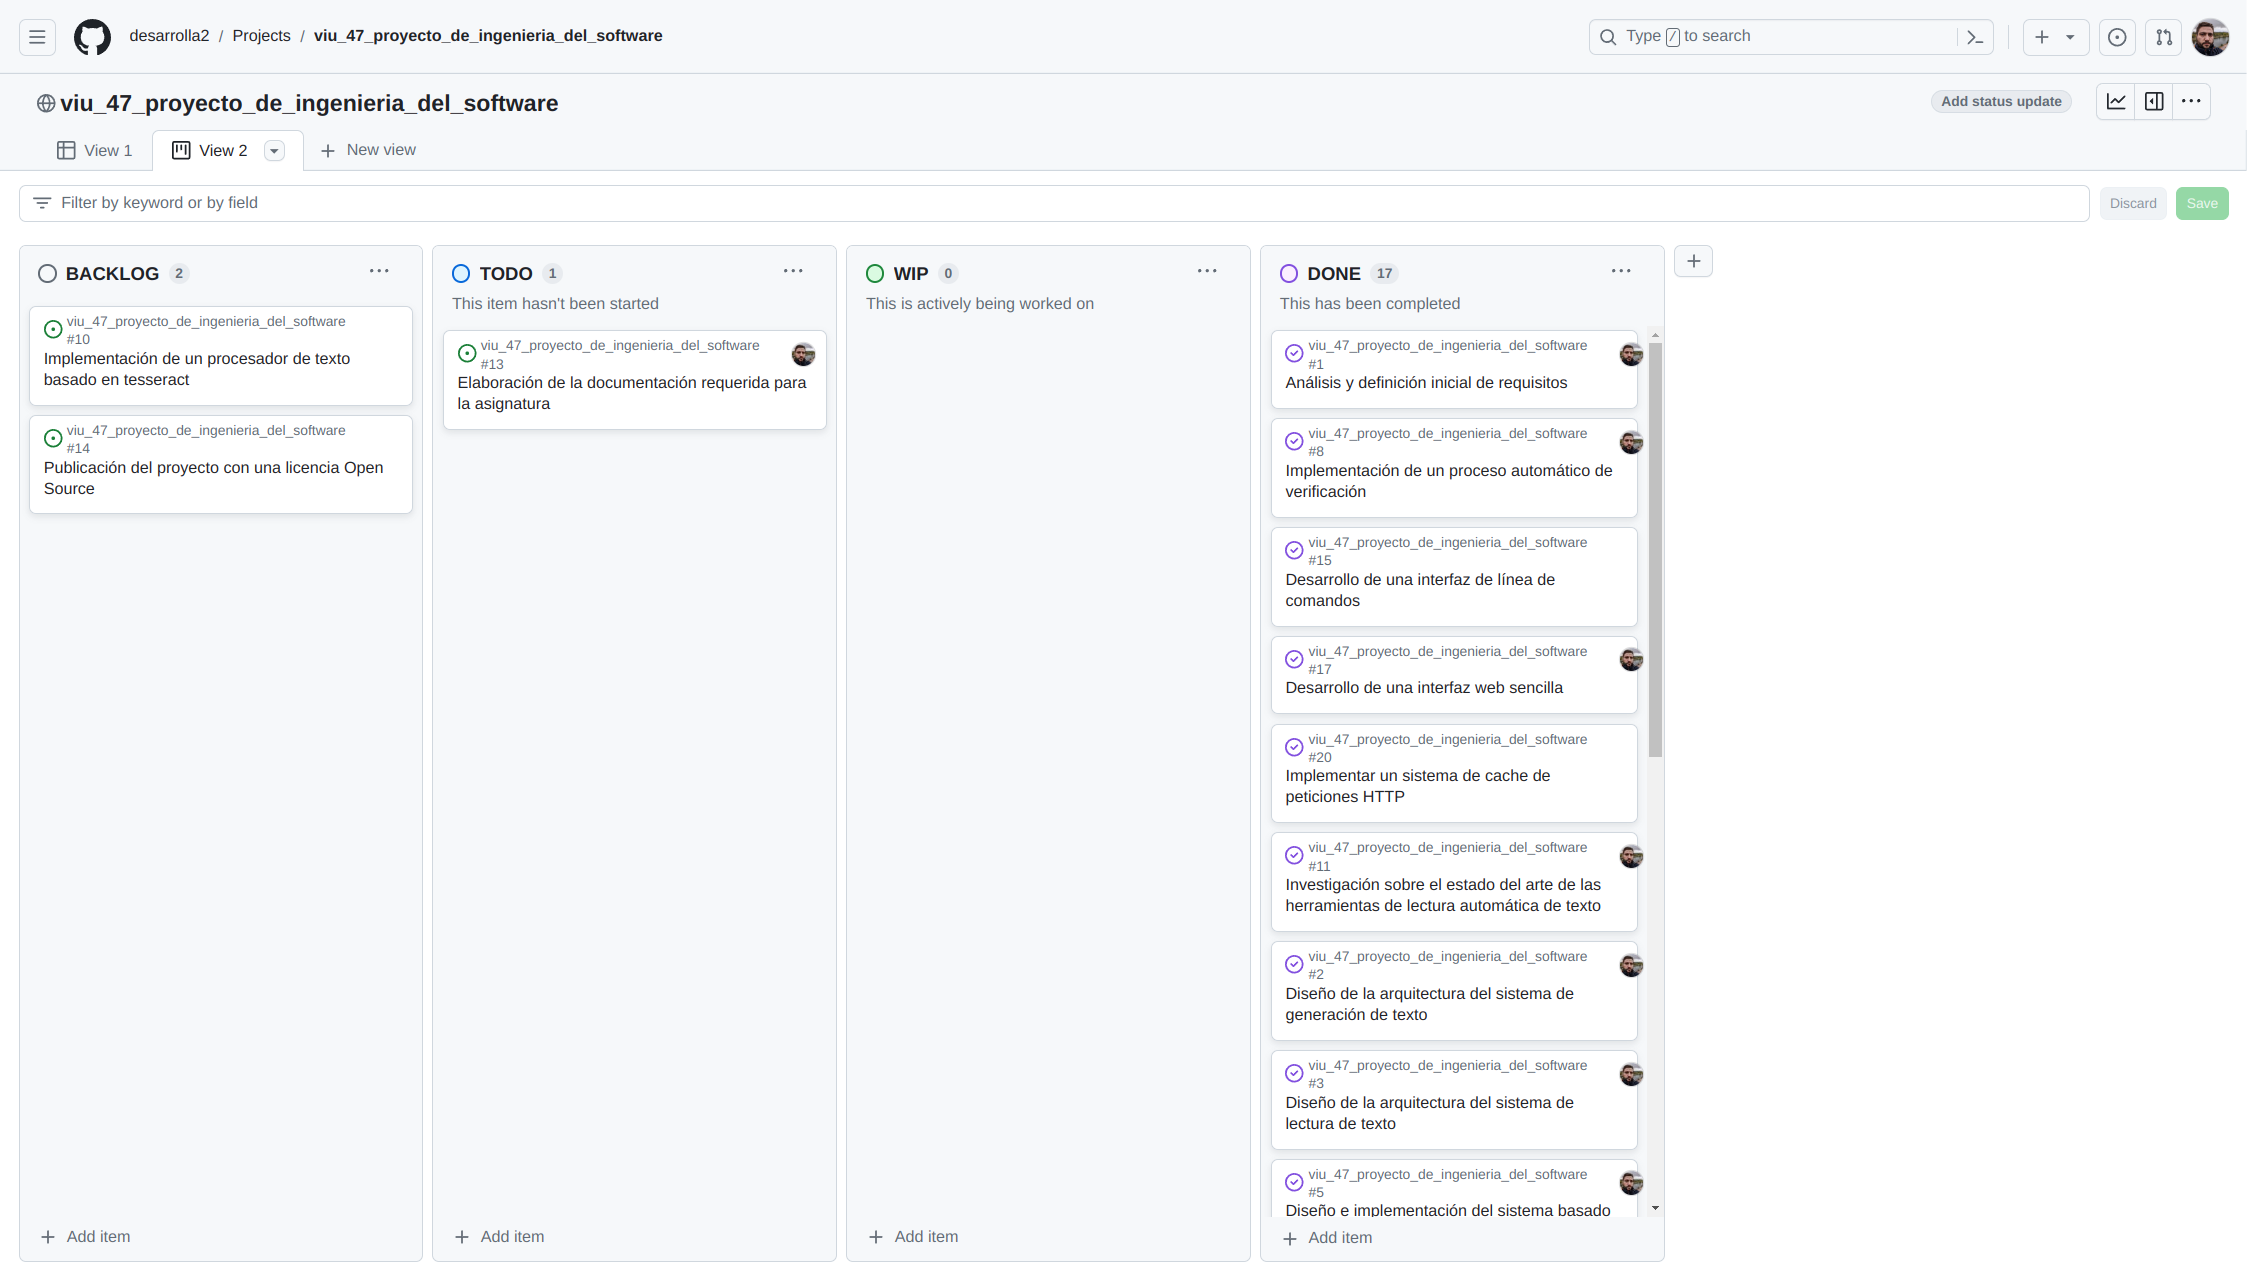
\includegraphics[width=\textwidth]{./chapter/3/images/chapter_3.kanban}
        \caption{Captura del tablero kanban del proyecto}
        \label{fig:chapter_3.kanban}
    \end{center}
\end{figure}

\textit{Kanban} promueve la mejora continua, la flexibilidad y la eficiencia, ayudando a los equipos a gestionar el
flujo de trabajo y a identificar cuellos de botella rápidamente.

En la figura~\ref{fig:chapter_3.kanban} puede una captura de cómo hemos usado \textit{kanban} para la gestión de las
tareas, teniendo en todo momento una visión completa del estado de avance de cada \textit{iteración}.

Al inicio del proyecto las tareas fueron definidas e incluidas en la columna \textbf{backlog}.
Durante el desarrollo del proyecto, si una nueva tarea era identificada, se incluía dentro de esta columna.

Al inicio de cada iteración, se realiza una planificación donde algunas tareas son incluidas dentro de la iteración
y las tareas son desplazadas a la columna \textbf{todo}.
Estas tareas deben encontrarse correctamente definidas y claras y el volumen total del trabajo debe estar adecuado a
la capacidad del equipo y del tiempo disponible en la iteración.

Durante la iteración las tareas se van desplazando a la columna \textbf{WIP} o \textit{work in progress} para
indicar que están siendo realizadas en este momento y finalmente a la columna \textbf{DONE}, una vez que son
completadas.

Al terminar cada iteración, todo el trabajo no completado, se desplaza de nuevo al \textit{backlog}.
Se realizan dos ceremonias, en una denominada \textit{demo} o demostración se realiza una demostración del trabajo
realizado, mientras que en la segunda, la \textit{retrospectiva} se realiza un análisis de los puntos fuertes y
puntos débiles del proceso de trabajo, con el objetivo de mitigar cualquier problema que pudiera surgir.

A modo de ejemplo añado los videos de ejemplo de una planificación~\cite{url_viu_47_proyecto_ingenieria_sprint_6_plan},
una demo~\cite{url_viu_47_proyecto_ingenieria_sprint_6_demo} y una
retrospectiva~\cite{url_viu_47_proyecto_ingenieria_sprint_6_retrospectiva} de la asignatura Proyecto de Ingeniería del
Software.
